\documentclass[osajnl,twocolumn,showpacs,superscriptaddress,10pt]{revtex4-1}


%PAQUETES<<<<<<<<<<<<<<<<<<<<<<<<<<<<<<<INICIO
\usepackage{dcolumn}% Align table %columns on decimal point
\usepackage{bm}% bold math
%
%Paquete de Idioma
\usepackage[spanish]{babel}
%
%Codificación Alfabeto
\usepackage[utf8]{inputenc}
%
%Codificación de Fuente
\usepackage[T1]{fontenc}
%
%Índice
\usepackage{makeidx}
%
%Gráficos3
\usepackage{graphicx}
\usepackage{subfig}
% \usepackage{longtable}
%\usepackage{xcolor} 
%
%Matemática
\usepackage{amsmath}
\usepackage{amsfonts}
\usepackage{amssymb}
%\usepackage{amstext} 
%
%Estilo de Página Numeración superior
%\pagestyle{headings}
%
%Hiperlinks \href{url}{text}
\usepackage[pdftex]{hyperref}
%
%Graficos y tablas
\usepackage{multirow}
%\usepackage{multicol}
\usepackage{float}
\usepackage{booktabs}
%
\decimalpoint
%\bibliographystyle{IEEEtran}
%\bibliography{IEEEabrv,mybibfile}
%
%
%PAQUETES<<<<<<<<<<<<<<<<<<<<<<<<<<<<<<<INICIO

\begin{document}
%SIGNOS
%TILDE -> \' <vocal>
%TEXTO_NEGRITA -> \textbf{<texto>}
%TEXTO_ITALICA -> \textit{<texto>}
%TEXTO_SUBRAYADO -> \underline{<texto>}

%TITTULO DEL ARTICULO
\title{\Huge IoT Práctica Uno -  Banda Inteligente - Arquitectura de Computadores y Ensambladores 2 }
%AUTORES DEL ARTICULO

\author{\newline Airton Yelstin de León Obando (201602836) - Rol: Analítico}
\affiliation{Grupo No.15 - Universidad de San Carlos de Guatemala, Escuela de Ciencias y Sistemas
}%

\author{\newline Oswaldo Giovanni Cáceres Samayoa, (201314164) - Rol: Conectividad}%
\affiliation{Grupo No.15 - Universidad de San Carlos de Guatemala, Escuela de Ciencias y Sistemas
}%
\author{\newline Anggelo Santiago Son Mux, (201709502) - Rol: Conectividad}%
\affiliation{Grupo No.15 - Universidad de San Carlos de Guatemala, Escuela de Ciencias y Sistemas
}%
\author{\newline Byron Gerardo Castillo Gómez, (201700544) - Rol: Smart-APP}%
\affiliation{Grupo No.15 - Universidad de San Carlos de Guatemala, Escuela de Ciencias y Sistemas
}%
\author{\newline Cristian Alberto Suy Mejia, (201700918) - Rol: Infraestructura}%
\affiliation{Grupo No.15 - Universidad de San Carlos de Guatemala, Escuela de Ciencias y Sistemas
}%
\date{Febrero 2021}



%INICIO DE DOCUMENTO<<<<<<<<<<<<<<<<<<<<<<<<<<<<<<<<<
\begin{abstract}
\title {resumen}
En esta pr\'actica se pretende hacer uso del concepto de Internet de las Cosas ( IoT - Internet of Things ) aplicado a una banda inteligente. Este banda se diseño de tal forma que sea capaz de transmitir informaci\'on de manera inmediata del estado del atleta al dispositivo de este mismo, lo anterior por medio de diferentes dispositivos electrónicos y sensores, adem\'as de un microcontrolador que recolecta la informaci\'on y la transmite a la nube. Todo lo anterior de manera que el usuario final tiene informaci\'on actualizada de su sobre su estado desde su dispositivo m\'ovil en cualquier momento y lugar.
\end{abstract}
\maketitle{}
\section{INTRODUCCIÓN}
Al hablar de introducir el concepto de IoT es este proyecto principalmente se habla de la importancia de recolectar datos y hacer uso de estos datos provenientes de cualquier objeto de la vida diaria cuya utilidad aumenta significativamente al convertir estos datos en información relevante y de interés en su funcionamiento, de tal manera que este objeto expande sus funciones para las que fue originalmente creado. Esta banda inteligente fue diseñado para proveer una solución a aquellos atletas o deportistas que buscan mantener monitoreados sus signos vitales y tener control sobre las actividades que realizan. Debido a lo anterior esta banda inteligente es capaz de realizar medidas de actividad del ritmo cardiaco, nivel de oxigeno, temperatura y todo gracias a un conjunto de diferentes dispositivos y sensores instalados en al banda que funcionarán en conjunto, la banda inteligente tiene la capacidad obtener el estado de las atleta en tiempo real, mientras realiza sus actividades deportivas, además no solo podrá saber los números sobre su estado sino también podrá obtener gráficas e historial sobre su actividad reciente tanto desde su dispositivo móvil como desde una aplicación web, en cualquier lugar y en cualquier momento. La comunicación es posible a través de una aplicación para dispositivos móviles con conexión a internet, conexión bluethoot e información proveniente la nube.

\section{Prototipo de Diseño}
Considerando que el propósito de este objeto es monitorear el estado del usuario se utiliza una banda para la muñeca, a continuación se puede apreciar un prototipo del objeto, observar Figura 1.


\begin{figure} [H] \centering 
\caption{Boceto de diseño}

\includegraphics[width=0.5\textwidth]{} 
Las dimensiones son de 
\end{figure}

\section{Famework de Productos Inteligentes Conectados}
\subsection{Infraestructura del Producto}
\subsubsection{Hardware:}
\begin{itemize}
    \item[$\bullet$]\textbf{Banda} para medidora.
    \item[$\bullet$]Dispositivo de \textbf{Módulo Bluethoot}.
    \item[$\bullet$]\textbf{Arduino.}
    \item[$\bullet$]\textbf{Cables} para conexiones.
    \item[$\bullet$]\textbf{Cautín} para realizar soldaduras.
    \item[$\bullet$]\textbf{Estaño.}
\end{itemize}
\subsubsection{Software}
    Se han diseñado y programado los algoritmos para la recolección de datos sobre el estado del cuerpo del usuario a traves de sensores y procesados con la ayuda de un microcontrolador ARDUINO para su posterior trasmisión a la nube.
    
\subsection{Sensores}
\begin{itemize}
    \item[$\bullet$]\textbf{Sensor de temperatura} para determinar la temperatura corporal del usuario.
    \item[$\bullet$]\textbf{Sensor ...} medir el ritmo cardiaco y niveles de oxigeno del usuario.
\end{itemize}
\subsection{Conexión}
    La comunicación a utilizar entre la banda inteligente y el usuario será a través de conexión \textbf{Bluethoot}. El dispositivo arduino recolecta la información para ser transmitida desde el módulo \textbf{Bluethoot} a el dispositivo móvil, este a su vez realiza peticiones \textbf{HTTP} con el servidor a través de una \textbf{API/REST} que se encargará de transmitir la información al dispositivo móvil del usuario. Ver figura 2. \newline
\begin{figure} [H] \centering 
\caption{Representación de conexión}

\includegraphics[width=0.5\textwidth]{} 
\end{figure}
\subsection{Análisis}
    Para este proyecto solamente se requiere que el buzón desinfecte los paquetes entregados una vez están dentro del compartimiento del buzón, además este producto de IoT debe informar al usuario sobre nuevos paquetes, estado de las puertas del buzón y nivel de líquido desinfectante y por lo tanto \textbf{no es necesario aplicar análisis en este proyecto.}
\subsection{Smart APP}
    Ya que el usuario deberá tener acceso al estado de sus lecturas e historial de actividad de la banda inteligente en todo momento se ha de ha desarrollado una aplicación inteligente para dispositivos móviles. Esta aplicación es compatible con dispositivos que utilizan el Sistema Operativo \textbf{Android}, entre algunas de sus funcione mas destacadas esta el dash-board con la actividad, a continuación se pueden apreciar las pantallas que muestran su funcionamiento:
    
\begin{figure} [H] \centering 
\caption{PANTALLA 1 ( Aplicación móvil )}
\includegraphics[width=0.4\textwidth]{} 
\end{figure}
\\
Cuando el buzón ha detectado un nuevo paquete en el compartimiento la aplicación muestra una advertencia al usuario sobre ello. Al seleccionar vera más información sobre ello.

\begin{figure} [H] \centering 
\caption{PANTALLA 2 ( Aplicación móvil )}
\includegraphics[width=0.4\textwidth]{} 
\end{figure}
\\
Una vez el buzón inteligente ha reconocido que se ha introducido un nuevo paquete la aplicación actualizara su estatus en la pantalla principal indicando la información de interés. Si hay un objeto mostrará un número uno de lo contrarios un número cero, además el peso del objeto y si se desea ver más solo debe presionar el botón \textbf{Get Data}.

\begin{figure} [H] \centering 
\caption{PANTALLA 3 ( Aplicación móvil )}
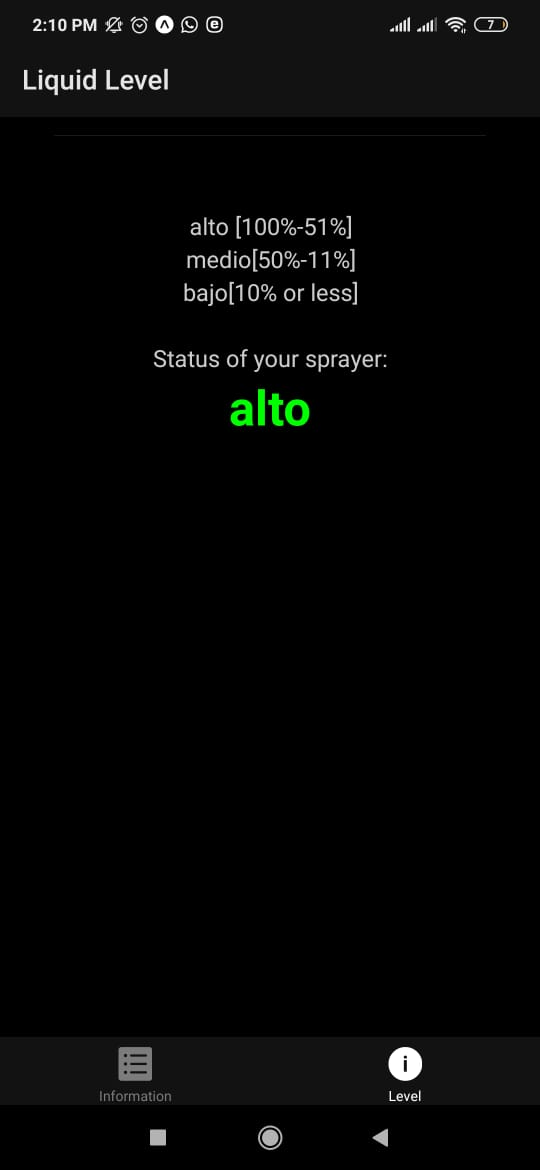
\includegraphics[width=0.4\textwidth]{img3.jpeg} 
\end{figure}
\\
Una vez se ha presionado el botón \textbf{Get Data}  el usuario puede ver la información detallada junto con el nivel de liquido desinfectante.

\section{Vídeos de funcionamiento}
\begin{itemize}
    \item[$\bullet$]Video1: https://youtu.be/1RXLjeAWD9k 
    \item[$\bullet$]Video2: https://youtu.be/fiz1PkFIdJ8
    \item[$\bullet$]Video3: https://youtu.be/uYKBNuGgTSc
\end{itemize}





\end{document}
